\relatorio
{Close Elections e Canais de Combate à Violência Contra a Mulher}
{

    \noindent \textbf{Políticas Públicas}
    
    \noindent Pesquisadores: Ana Beatriz Parra Ferreira, Antônio Vicente Fernandes de Andrade, Maria Fernanda Pizarro Carvalho
    
    \noindent Orientador: Adriano Dutra Teixeira

}
{

   Estudo sobre o efeito da representação política feminina em políticas de combate à violência doméstica. Análise do papel da Delegacia Especializada de Atendimento à Mulher (DEAM) como um canal de combate à violência contra a mulher. Como metodologia, foi utilizada uma Regressão Descontínua (RDD) aplicada em Close Elections. 

}
{
Close Elections, Prefeitas, Violência Doméstica
}

% ------ INICIO RELATORIO -------


  
\section{Introdução}
\label{introducao}

A violência contra a mulher é um grave problema social e de saúde pública no Brasil. As manifestações de violência contra a mulher não se limitam apenas às agressões físicas, abrangendo também diferentes formas de violência psicológica, emocional, patrimonial e financeira. Tais violências podem ser analisadas em relação ao espaço de ocorrência, manifestando-se tanto no âmbito privado quanto no público. Em todos os casos, o gênero é o fator comum que as caracteriza, seja em contextos familiares ou em relações de natureza pública, uma vez que as questões subjacentes a essas violências são, fundamentalmente, questões de gênero, envolvendo mulheres ou problemas considerados ``femininos'' pela cultura vigente \cite{schraiber2005violencia}. 

% [add algo aqui]


Nesse contexto, a promoção do bem-estar feminino em face da violência exige a avaliação dos recursos destinados à mitigação desse fenômeno. A análise da efetividade dos canais de combate à violência contra a mulher, e, em particular, o conhecimento específico sobre esses canais, torna-se de extrema importância e motiva a presente pesquisa. Assim, como será detalhadamente abordado na Seção \ref{Modelagem_teorica}, a participação feminina na política será utilizada para embasar a avaliação de um canal de combate à violência contra a mulher: as Delegacias Especializadas de Atendimento à Mulher.

\subsection{Representação feminina e seu papel no Combate a Violência de Gênero}
\label{representacao_feminina}

É importante trazer à tona a representatividade nos espaços públicos e de liderança no Brasil. A representatividade feminina já é explorada na academia. O paper ``Future electoral impacts of having a female mayor'' explora como o Brasil elegeu, ao longo das últimas eleições, cada vez mais mulheres para cargos de prefeitas e como o desempenho positivo das mesmas contribuiu para a eleição de mais mulheres se tornando deputadas e governadoras em eleições federais \cite{arvate2017future}. Os resultados do estudo têm implicações para a compreensão de como a eleição de líderes femininas afeta a representação política das mulheres e o potencial de ameaça de estereótipo e voto com viés de gênero.

Consoante à isso, existem evidências sobre o efeito das mulheres na política em índices de violência. O paper ``Fighting violence against women: The role of female political representation'', apresenta o feito da gestão de uma prefeita nos casos de violência doméstica em municípios brasileiros \cite{bochenkova2023fighting}. Conclui-se que em municípios em que a pessoa eleita é mulher, os casos de violência contra as mulheres diminuem, em média, em 50\%. Este resultado foi obtido através de uma metodologia que faz uso de uma regressão descontínua, que será utilizada nesta pesquisa e aprofundada na seção \ref{rdd}. 

A partir dos estudos sobre a participação de mulheres e sua influência na redução de violência feminina, alguns questionamentos são alavancados, como ``Quais são os principais canais de combate à violência doméstica?" ou ``Quais destes canais são utilizados pelas prefeitas para a redução da violência?". Responder tais perguntas não é uma tarefa trivial e envolve avaliar diversos possíveis canais de combate, sendo um procedimento que extrapola o escopo da seguinte pesquisa. Dessa forma, o proposta deste estudo é avaliar a efetividade de um provavel canal de combate à violência contra a mulher, a Delegacia Especializada de Atendimento à Mulher, detalhada na seção \ref{DEAMs}. 

\subsection{ Delegacia Especializada de Atendimento à Mulher (DEAMs)}
\label{DEAMs}
% [ DESCREVER DEAMS]

As Delegacias Especializadas de Atendimento à Mulher (DEAMs) são unidades brasileiras da Polícia Civil criadas com o objetivo específico de oferecer atendimento especializado e acolhedor para mulheres vítimas de violência doméstica, física, psicológica, sexual, patrimonial e outras formas de abusos. 

As DEAMs buscam não apenas a resolução de crimes, mas também a promoção da autonomia das mulheres, oferecendo apoio jurídico, psicológico e social, com o intuito de romper o ciclo de violência e garantir a proteção das vítimas. Criadas pelos governos estaduais a partir de 1985, as DEAMs constituíram-se, até recentemente, na principal, senão muitas vezes a única, política pública de prevenção e combate à violência contra as mulheres \cite{silva2012deams}. 

Evidências na literatura apresentam o impacto da implementação de Delegacias Especializadas de Atendimento a Mulher nas taxas de abusos e agressões que acontecem em relações românticas, chamadas formalmente de Intimate Partner Violence (IPV). O paper ``Women's police stations and intimate partner violence: Evidence from Brazil” realisa essa avaliação fazendo uso de um \textit{staggered Diff-in-Diff}, comparando os municípios que implementaram e que não implementaram as delegacias \cite{perova2017women}. 

O estudo conclui que embora não se encontre uma forte associação média, as DEAMs demonstram ser altamente eficazes entre mulheres jovens que vivem em áreas metropolitanas. Estabelecer uma DEAM em um município metropolitano está associado a uma redução na taxa de homicídios femininos de 1,23 mortes por 100.000 mulheres de 15 a 49 anos - aproximadamente uma redução de 17\% na taxa de homicídios femininos grandes cidades. Paralelamente, a redução na taxa de homicídios de mulheres de 15 a 24 anos é ainda maior: 5,57 mortes por 100.000 mulheres. 

Concatenando a conclusões dos estudos apresentados em \ref{representacao_feminina} e \ref{DEAMs}, as ponderações construídas até o momento embasam a hipótese deste estudo: \textbf{``A implementação de Delegacias Especializadas em Atendimento a Mulher (DEAMs) é um canal de combate à violência doméstica no mandato de prefeitas?”}

\section{Modelagem Teórica}
\label{Modelagem_teorica}

Na literatura econômica, a unidade familiar é comumente vista como uma unidade cooperativa, na qual os agentes buscam maximizar a utilidade do núcleo familiar de forma ``altruísta''.  Entretanto, famílias acometidas pela violência doméstica se encaixam mais adequadamente em um jogo estratégico, no qual cada parceiro busca maximizar a própria utilidade, sujeito à restrição de que o cônjuge permaneça na relação. \cite{farmer1997economic}. 

É importante frisar que o modelo em questão aborda um contexto presente em unidades familiares tradicionais e que seguem um raciocínio de papéis de gênero que, na contemporaneidade, pode ser visto como obsoleto em outras dinâmicas familiares. 

Para entender quais fatores impactam na tomada de decisão dos sujeitos que compõem esta unidade familiar é necessário olhar para as funções de utilidade e restrições orçamentárias de cada cônjuge. Nesta analise econômica da violência domestica, duas importantes tomadas de decisão têm grande importância: a decisão de quanta violência será aplicada pelo cônjuge e a decisão de terminar o casamento por parte da mulher. Essas tomadas de decisão são reflexões das utilidades de cada cônjuge dentro de um casamento.  

No contexto desse modelo, a utilidade refere-se à satisfação ou bem-estar que cada indivíduo obtém das decisões e ações dentro do relacionamento. Cada pessoa tenta maximizar sua utilidade, tomando decisões sobre como agir em relação ao outro, levando em consideração tanto os custos quanto os benefícios de suas escolhas.
 
\subsection{Utilidade do Homem}

No modelo, o homem busca maximizar sua utilidade ao interagir com a mulher de uma forma que beneficie seus próprios interesses. Isso pode incluir fatores como controle, poder, ou acesso a recursos dentro do relacionamento. Se o homem acredita que pode aumentar sua utilidade ao exercer controle sobre a mulher — incluindo o uso da violência — ele pode ser incentivado a praticá-la, especialmente se o custo da violência for percebido como baixo (ou seja, se ele acredita que não haverá consequências significativas para suas ações).

A utilidade do homem também está associada à manutenção da relação, à obtenção de benefícios materiais, emocionais ou sociais, e ao controle sobre a mulher, que pode ser interpretado como uma forma de garantir a estabilidade de suas próprias necessidades e interesses. No entanto, é importante notar que, no modelo, a utilidade do homem pode ser afetada por diversas variáveis, como os custos da violência (se houver punições ou problemas sociais associados a ela) e as alternativas disponíveis fora do relacionamento.

Primeiramente, a função utilidade do homem é definida como:

\begin{equation}
    U^M = U^M(S(V),C^M,\eta)       
\label{eq:utilidade_homem}
\end{equation}

Em que $S(V)$ representa uma função autoestima que agrega utilidade quando o sujeito reforça uma relação de poder sobre sua parceira através, por exemplo, da violência $(V)$ empregada sobre ela. O $\eta$ representa o benefício matrimonial, isto é, o benefício de se manter no casamento, e $C^M$ representa o consumo desse indivíduo que deriva, naturalmente, de sua restrição orçamentária que é definida pelas equações \ref{eq:ro_homem} e \ref{eq:ro_homem_consumo}.

\begin{equation}
I^M - t^M = P_c * C^M
\label{eq:ro_homem}
\end{equation}

\begin{equation}
C^M = \frac{I^M - t^M}{P_c}
\label{eq:ro_homem_consumo}
\end{equation}

A igualdade na restrição orçamentaria (\ref{eq:ro_homem}) indica que o sujeito só gastará aquilo que ele é capaz de gastar. Ou seja, seu gasto total $(P_c * C^M)$ será igual sua renda líquida $(I^M - t^M)$. Aqui, $I^M$ representa sua renta bruta, $t^M$ representa as transferências que o sujeito faz para a esposa, como arcar com as contas da casa, por exemplo, $Pc$ é o preço da cesta de consumo e $C^M$ é o seu consumo em si.

Isolando o consumo ($C^M)$ em (\ref{eq:ro_homem_consumo}), e o substituindo-o em (\ref{eq:utilidade_homem}), temos a função utilidade completa desse indivíduo:

\begin{equation}
U^M = U^M(S(V),\frac{I^M - t^M}{P_c},\eta)       
\label{eq:utilidade_homem_completa}
\end{equation}

\subsection{Utilidade da Mulher}

Para a mulher, a utilidade está ligada à satisfação e segurança que ela obtém dentro do relacionamento, que pode incluir aspectos como afeto, apoio emocional e segurança financeira. No entanto, o modelo também considera os custos associados à violência doméstica, que afetam negativamente sua utilidade. A mulher pode ser levada a aceitar ou até mesmo a justificar a violência em certos casos, se acreditar que os benefícios da relação superam os custos da agressão, ou se não perceber alternativas viáveis para escapar do abuso (por exemplo, devido à dependência financeira ou medo de retaliações).

Além disso, a utilidade da mulher pode ser moldada pela percepção do risco e pelas normas sociais em torno da violência. Se a mulher acredita que a violência é uma parte aceitável de um relacionamento ou se as instituições não oferecem um suporte adequado, sua utilidade pode ser negativamente impactada, mas ela pode não ter as condições para mudar essa dinâmica.

Analogamente, a utilidade da mulher segue uma distribuição semelhante à do homem, 

\begin{equation}
    U^W = U^W(V, C^W, \eta, U^M)
\label{eq:utilidade_mulher}
\end{equation}

com o seu consumo $(C^W)$ e o benefício matrimonial $(\eta)$ presentes. As principais diferenças são que agora, ao invés de uma função autoestima, a violência empregada entra diretamente no cálculo da utilidade de forma negativa $(V)$ e que a utilidade do homem entra no bem estar da mulher. 

\begin{equation}
    I^W + t^W = P_c * C^W
   \label{eq:ro_mulher} 
\end{equation}

\begin{equation}
    C^W = \frac{I^W + t^W}{P_c}
    \label{eq:ro_mulher_consumo}
\end{equation}

\begin{equation}
    U^W = U^W(V, \frac{I^W + t^M}{P_c}, \eta, U^M(S(V),\frac{I^M - t^M}{P_c},\eta))
    \label{eq:utilidade_mulher_completa}
\end{equation}

Outra diferença está na restrição orçamentária da mulher $(\ref{eq:ro_mulher})$, com as transferências do homem agora adicionando à sua renda líquida. Isolando o consumo em (\ref{eq:ro_mulher_consumo}) e substituindo (\ref{eq:ro_mulher_consumo}) e (\ref{eq:utilidade_homem_completa})
em (\ref{eq:utilidade_mulher}) chegamos na equação completa da utilidade da mulher no casamento (\ref{eq:utilidade_mulher_completa}).

\subsection{Ponto de Ameaça}

O principal ponto da análise é que a mulher, além da utilidade no casamento, pondera a sua utilidade enquanto solteira para tomar a decisão de se manter, ou não, no casamento. O ponto de ameaça da mulher, ou seja, a sua utilidade fora do casamento $(\overline{U}^W(C_S^W))$ é uma função do consumo da mulher fora do casamento, que segue, naturalmente, uma outra restrição orçamentária:

\begin{equation}
    I^W + X = P_C * C_S^W
\label{eq:ro_solteira}
\end{equation}

\begin{equation}
C_S^W = \frac{I^W + X}{P_C}
\label{eq:ro_solteira_consumo}
\end{equation}

\begin{equation}
\overline{U}^W(\frac{I^W + X}{P_C})
\label{eq:ponto de ameaça}
\end{equation}

Observa-se, em \ref{eq:ro_solteira}, que agora as transferências de renda do marido já não entram na restrição orçamentária da mulher. No lugar delas, tem-se o $(X)$, que representa a Rede de Apoio da mulher fora do casamento, ou seja, familiares ou serviços estatais que dão suporte à mulher caso ela se divorcie, por exemplo. 



\subsection{O Problema de Maximização}

Formalmente, o problema pode ser expresso da seguinte maneira:

\begin{equation}
\max_{\substack{V, C^M}} U^M(S(V), C^M, \eta)
\quad \text{s.a.} \quad U^W=U_S^W
\label{eq:max}
\end{equation}


A restrição imposta ao problema indica que a mulher só permanecerá no casamento caso sua utilidade dentro da relação seja pelo menos igual à sua utilidade de reserva.

A resolução do problema de maximização, utilizando a técnica do Lagrangeano, conduz a dois resultados fundamentais:

\begin{equation}
\frac{U_V^M}{U_C^M} = -\frac{U_V^W}{U_C^W} 
\label{eq:resultado_1}
\end{equation}
 
\begin{equation}
U^W = \overline{U}^W
\label{eq:resultado_2}
\end{equation}

O primeiro resultado, equação (\ref{eq:resultado_1}), evidencia que, no equilíbrio, as taxas marginais de substituição entre violência e consumo para ambos os cônjuges são iguais em módulo, mas de sinais opostos. Isso significa que um aumento na violência imposta pelo homem gera uma necessidade proporcionalmente maior de compensação em consumo para a mulher, de modo que ela aceite continuar na relação. Esse equilíbrio pode ser visualizado graficamente na Figura \ref{fig:micro1}.

\begin{figure} 
    \centering
    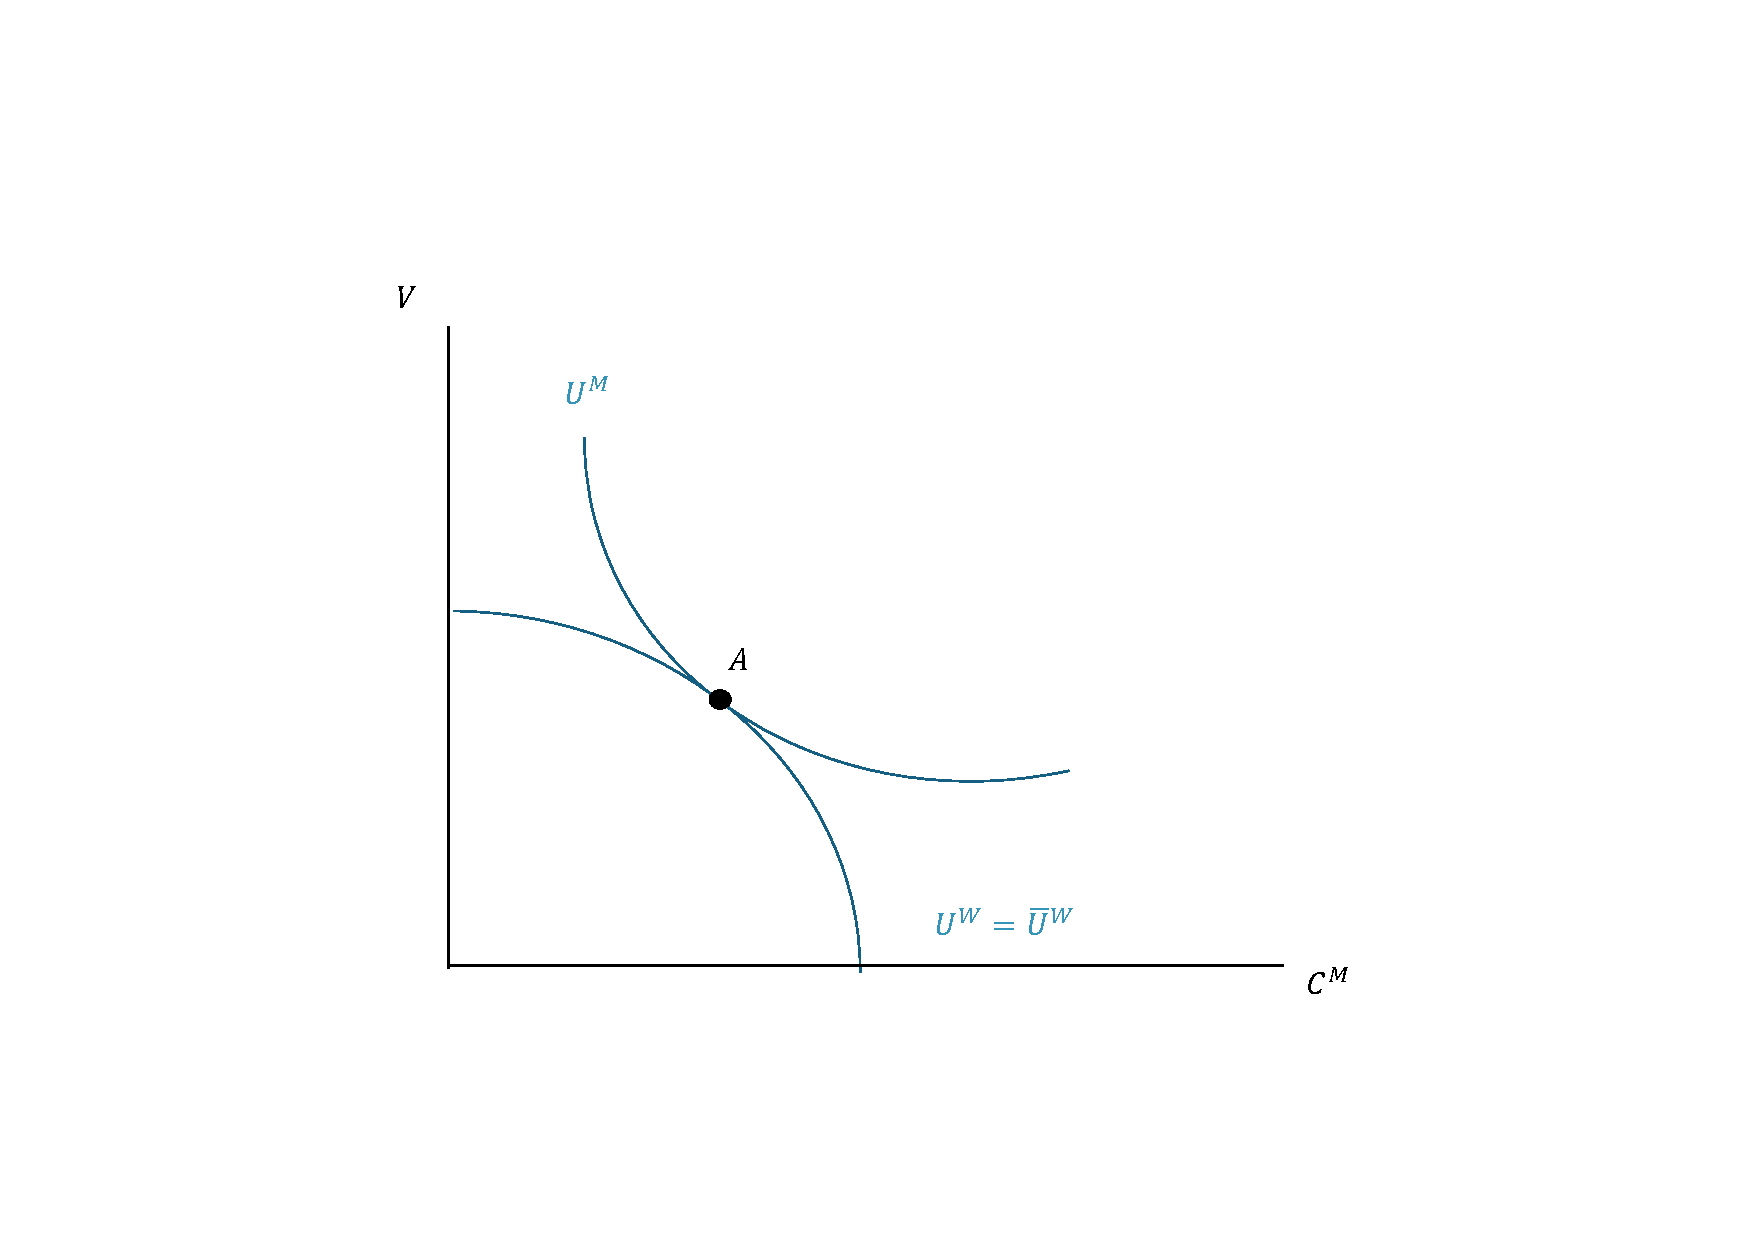
\includegraphics[width=0.8\linewidth]{relatorios/close_elections/graficos/micro1.pdf}
    \caption{Representação gráfica do equilíbrio inicial}
    \label{fig:micro1}
\end{figure}

\begin{figure} 
    \centering
    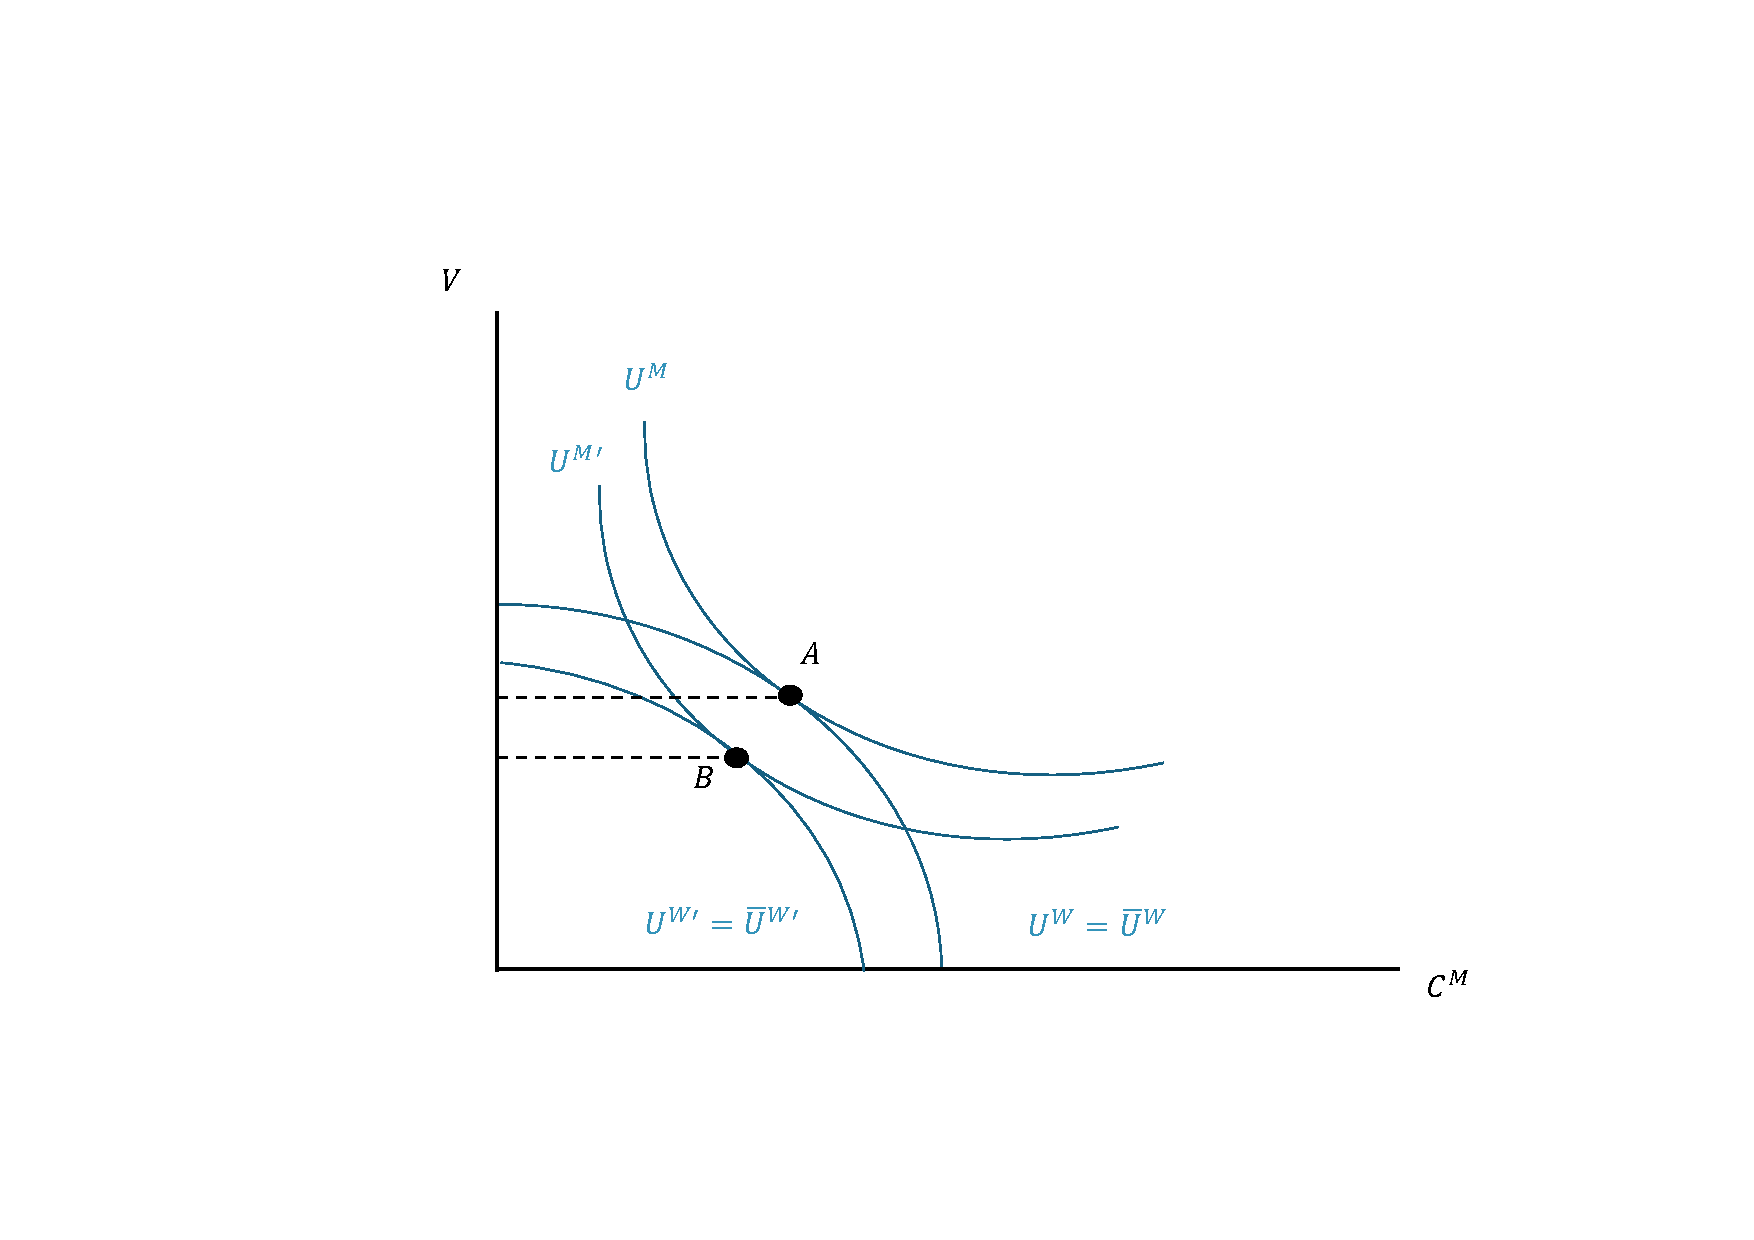
\includegraphics[width=0.8\linewidth]{relatorios/close_elections/graficos/micro2.pdf}
    \caption{Deslocamento do equilíbrio após o aumento da rede de apoio}
    \label{fig:micro2}
\end{figure}

O segundo resultado, equação (\ref{eq:resultado_2}), indica que a utilidade da mulher se mantém exatamente no limite da sua utilidade de reserva. Caso ocorra qualquer alteração que aumente essa utilidade externa ao casamento, como o fortalecimento de redes de apoio, o ponto de tangência na curva de equilíbrio se desloca.

\subsubsection{Impacto do Aumento da Rede de Apoio}

A presença de uma rede de apoio mais ampla e eficaz para a mulher altera a equação de equilíbrio. Na prática, isso reduz a quantidade de violência que ela está disposta a tolerar dentro da relação, tornando o divórcio uma opção mais viável. Esse efeito pode ser observado na Figura \ref{fig:micro2}, onde o novo ponto de equilíbrio se desloca para uma situação em que a mulher aceita níveis menores de violência antes de optar por sair do casamento.

\section{Modelagem Empírica}
\label{modelagem_empirica}



\subsection{Close Elections - Eleições Acirradas}
\label{close_elections}

A análise de Close Elections é fundamental para esta pesquisa, pois permite avaliar os impactos causais da competição eleitoral sobre políticas públicas e respostas institucionais, como a atuação das Delegacias Especializadas de Atendimento à Mulher (DEAMs). Em conjunto com a metodologia de Regressão Descontínua (RDD), discutida na Seção \ref{rdd}, eleições municipais em que a margem de vitória entre dois candidatos foi estreita foram utilizadas, de modo a explorar os efeitos da competitividade eleitoral.

O conceito de Close Elections baseia-se na intuição de que, à medida que a diferença de votos entre o vencedor e o perdedor se reduz, a eleição torna-se mais competitiva e seu resultado mais probabilístico \cite{grimmer2011close}. Isso significa que, em disputas muito acirradas, pequenas variações no comportamento do eleitorado podem determinar o vencedor, tornando o desfecho eleitoral quase aleatório. Esse fenômeno confere ao estudo de Close Elections um caráter de experimento natural, pois permite comparar contextos eleitorais semelhantes em que o único fator determinante da vitória foi uma pequena variação na votação.

A aleatoriedade inerente às eleições marginais é frequentemente utilizada como suposição estatística útil em inferência causal. Em um cenário com apenas dois candidatos, uma eleição altamente competitiva é aquela em que ambos possuem chances equivalentes de vencer. No limite, quando a margem eleitoral se aproxima de zero, o resultado pode ser interpretado como se fosse determinado pelo lançamento de uma moeda justa. Esse princípio embasa a metodologia de RDD, uma vez que torna as características individuais dos candidatos, partidos e distritos ortogonais ao desfecho eleitoral. Assim, é possível estimar efeitos causais de forma mais confiável, sem as preocupações usuais com endogeneidade que afetam estudos eleitorais convencionais \cite{grimmer2011close}.

Neste estudo, a seleção das eleições marginais foi realizada a partir dos microdados do Tribunal Superior Eleitoral (TSE), permitindo identificar disputas com pequenas margens de vitória. Adicionalmente, os dados foram combinados com registros administrativos de violência de gênero, provenientes do DataSUS e de órgãos governamentais, para investigar se mudanças políticas decorrentes de eleições acirradas afetam as taxas de violência doméstica e a atuação das DEAMs. Também foram construídas estatísticas descritivas para examinar o perfil dos candidatos e das eleições analisadas, incluindo a proporção de homens e mulheres concorrendo e a distribuição partidária dos candidatos. 

A abordagem baseada em Close Elections e RDD permite, assim, avaliar de maneira robusta os efeitos da competitividade eleitoral sobre políticas de enfrentamento à violência de gênero, minimizando problemas de viés de seleção e confundimento. Os resultados obtidos podem contribuir para um melhor entendimento sobre como disputas eleitorais influenciam decisões institucionais e políticas públicas voltadas para a proteção das mulheres.

\subsection{Regressão Descontínua - RDD}
\label{rdd}

A Regressão Descontínua (RDD) é uma metodologia econométrica amplamente utilizada para inferência causal em cenários onde existe um ponto de corte bem definido separando unidades tratadas e não tratadas. No contexto eleitoral, essa abordagem explora a descontinuidade gerada pela margem de vitória mínima em eleições acirradas para identificar efeitos causais da escolha de um candidato sobre diferentes desfechos políticos e sociais.

O principal pressuposto do RDD é que, ao redor do limiar de vitória, os municípios que elegeram um candidato e aqueles que elegeram seu adversário são comparáveis, pois pequenas variações na votação são essencialmente aleatórias. Isso permite que a eleição marginal funcione como um experimento natural, no qual se pode inferir o impacto da vitória de determinado grupo político sem os vieses normalmente presentes em estudos observacionais \cite{grimmer2011close}. 

Para garantir a validade da inferência causal, são adotadas técnicas como a escolha otimizada do \textit{bandwidth}, testes de balanceamento das covariáveis e análise de sensibilidade para verificar a robustez dos resultados. Além disso, gráficos de descontinuidade são utilizados para inspecionar visualmente os efeitos estimados, complementando a análise estatística.

Dessa forma, a aplicação do RDD nesta pesquisa permite isolar os efeitos da competição política sobre a violência de gênero e avaliar como mudanças no governo local impactam na efetividade das DEAMs em combater a violência doméstica.

A especificação da regressão é escrita da seguinte forma:

\begin{equation}
    y_{t,\mu} =  \beta_0 + \gamma D_g + f(Mv_\mu) + x^\mu_{t,\mu} +  x^p_{t,\mu} + \varepsilon_{t,\mu}
\end{equation}

Onde \(y_{t,\mu}\) representa o número de homicídios de mulheres no município \(\mu\) no período \(t\). O termo \(\beta_0\) denota o intercepto da equação, a variável \(D_g\) indica a eleição de uma mulher como prefeita, sendo um fator de interesse para o estudo, e \(\gamma\) representa justamente o efeito causal dessa variável sobre os homicídios de mulheres. A função \(f(Mv_\mu)\) captura a influência da margem de vitória entre prefeitas e prefeitos sobre os homicídios. Os termos \(x^\mu_{t,\mu}\) e \(x^p_{t,\mu}\) representam, respectivamente, conjuntos de características municipais e dos candidatos. \(\varepsilon_{t,\mu}\) é o termo de erro, que captura a variação nos homicídios de mulheres não explicada pelas variáveis do modelo.


\subsection{Dados}
\label{dados}

A pesquisa utiliza um conjunto de dados detalhado sobre eleições municipais no Brasil, combinando informações eleitorais com registros administrativos de violência de gênero. Os dados utilizados foram obtidos de diferentes fontes. 

As informações sobre eleições municipais foram extraídas da base de dados do Tribunal Superior Eleitoral (TSE), acessadas por meio da biblioteca \texttt{electionsBR}. Esses dados incluem o total de eleitores, a votação por candidato e as margens de vitória em diferentes pleitos. Para complementar a análise, foram incorporadas características socioeconômicas municipais obtidas a partir de bases do IBGE, permitindo controlar fatores estruturais que possam influenciar tanto os resultados eleitorais quanto os índices de violência. 

No que diz respeito aos dados de violência, a pesquisa utiliza registros de homicídios como proxy para a violência de gênero. Essa escolha se justifica pelo fato de que homicídios, especialmente feminicídios, são menos sujeitos à subnotificação em comparação a outros tipos de violência doméstica, como agressões e ameaças. Os dados de homicídios foram extraídos do sistema de informações do DataSUS, garantindo maior confiabilidade na mensuração do fenômeno analisado. 

Além disso, os dados sobre a atuação das Delegacias Especializadas de Atendimento à Mulher (DEAMs) foram obtidos por meio do Ministério da Mulher, a partir de um conjunto de informações disponibilizado por pesquisadoras contatados durante a realização deste projeto. Esses dados permitem avaliar a presença das DEAMs nos municípios ao longo do tempo. 

Os dados eleitorais foram processados para identificar eleições acirradas, definidas como aquelas em que a diferença de votos entre o vencedor e o segundo colocado está dentro de um intervalo específico. A variável de interesse, que mede a intensidade da competição eleitoral, será posteriormente utilizada na análise de regressão descontínua. Além disso, os registros de violência foram organizados de maneira a permitir a identificação de tendências antes e depois das eleições, viabilizando a avaliação de possíveis impactos das mudanças políticas na resposta institucional e na incidência de violência doméstica.

Foram realizadas diversas etapas de tratamento e limpeza. Primeiramente, foram selecionadas apenas eleições municipais com margem de vitória estreita, uma vez que esse critério permite uma análise mais robusta dos efeitos causais. Em seguida, os indicadores de violência foram normalizados, possibilitando a comparação entre diferentes municípios e ao longo do tempo. Por fim, as diversas fontes de dados foram integradas em uma única base consolidada, permitindo a realização de análises econométricas que associam os resultados eleitorais a mudanças nos padrões de violência e na resposta institucional das DEAMs.

A partir dessa base estruturada, o método de RDD foi aplicado para avaliar a relação entre a característica eleitoral e a atuação das DEAMs, bem como os impactos nas estatísticas de violência doméstica. 


\section{Resultados}

Aplicando as metodologias descritas na modelagem empírica, os resultados obtidos evidenciaram um impacto positivo da eleição de prefeitas na redução dos homicídios em ambientes domésticos. A estimação utilizando RDD permite identificar um efeito causal direto da representatividade feminina na política sobre a violência contra as mulheres.



A Tabela \ref{tab:resultados} apresenta os coeficientes estimados utilizando as variáveis de interesse homicídio doméstico e margem de vitória feminina nas eleições, mostrando que há uma redução estatisticamente significativa de aproximadamente 1,2 homicídios por 100 mil habitantes no mandato quando uma mulher é eleita prefeita.

\begin{table}[h]
    \centering
    \begin{tabular}{lccccc}
        \toprule
        \textbf{Método} & \textbf{Coef.} & \textbf{Erro Padrão} & \textbf{z} & \textbf{P-valor} & \textbf{[95\% C.I.]} \\
        \midrule
        Convencional    & -1.114 & 0.502 & -2.221 & 0.026 & [-2.097 , -0.131] \\
        Viés-Corrigido  & -1.246 & 0.502 & -2.483 & 0.013 & [-2.229 , -0.262] \\
        Robusto         & -1.246 & 0.566 & -2.199 & 0.028 & [-2.356 , -0.136] \\
        \bottomrule
    \end{tabular}
    \caption{Resultados da estimação por RDD para homicídios domésticos.}
    \label{tab:resultados}
\end{table}

A Figura \ref{fig:rdd_plot} ilustra essa descontinuidade na margem eleitoral, reforçando a hipótese de que a presença de prefeitas reduz a violência (homicídios) contra as mulheres. Observa-se uma quebra na tendência dos homicídios domésticos ao longo da margem de vitória feminina, sugerindo que a estimativa reflete um efeito causal válido, interpretado como um Local Average Treatment Effect (LATE) para os municípios próximos ao limiar de vitória eleitoral.


\begin{figure}
    \centering
    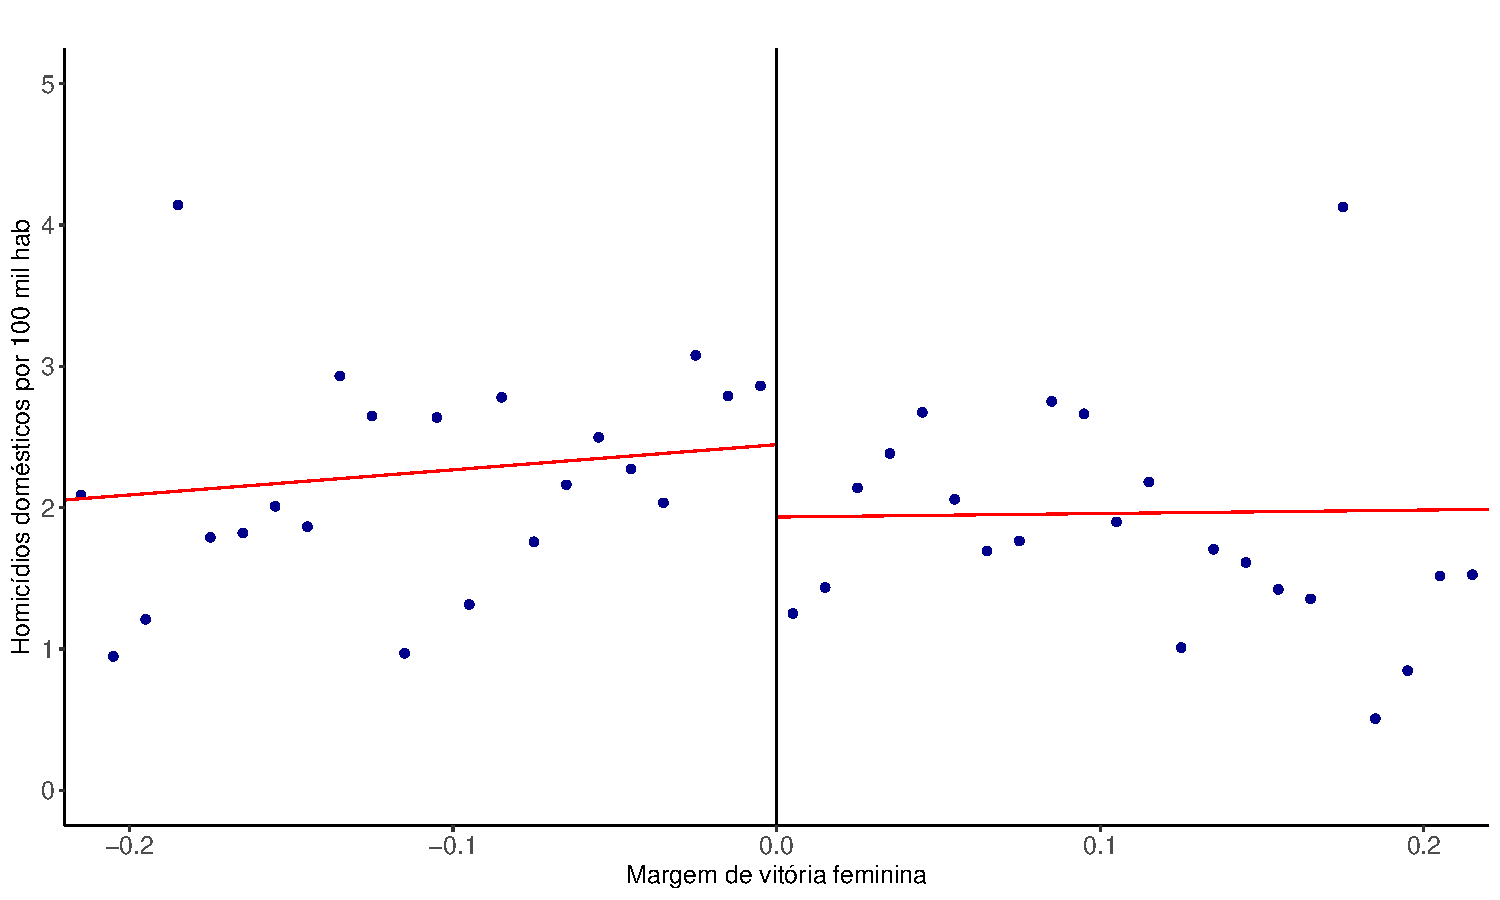
\includegraphics[width=0.8\linewidth]{relatorios/close_elections/graficos/rdd_plot.pdf}
    \caption{Visualização do RDD - Efeito da eleição de uma prefeita sobre homicídios domésticos.}
    \label{fig:rdd_plot}
\end{figure}

Para validar a robustez dessa relação causal, foi conduzido um teste placebo analisando o impacto da eleição em um período anterior, representado na Figura \ref{fig:rdd_plot_t_1}. Como esperado, o efeito não é significativo, indicando que a redução nos homicídios ocorre apenas após a eleição da prefeita, e não antes. 

\begin{figure}
    \centering
    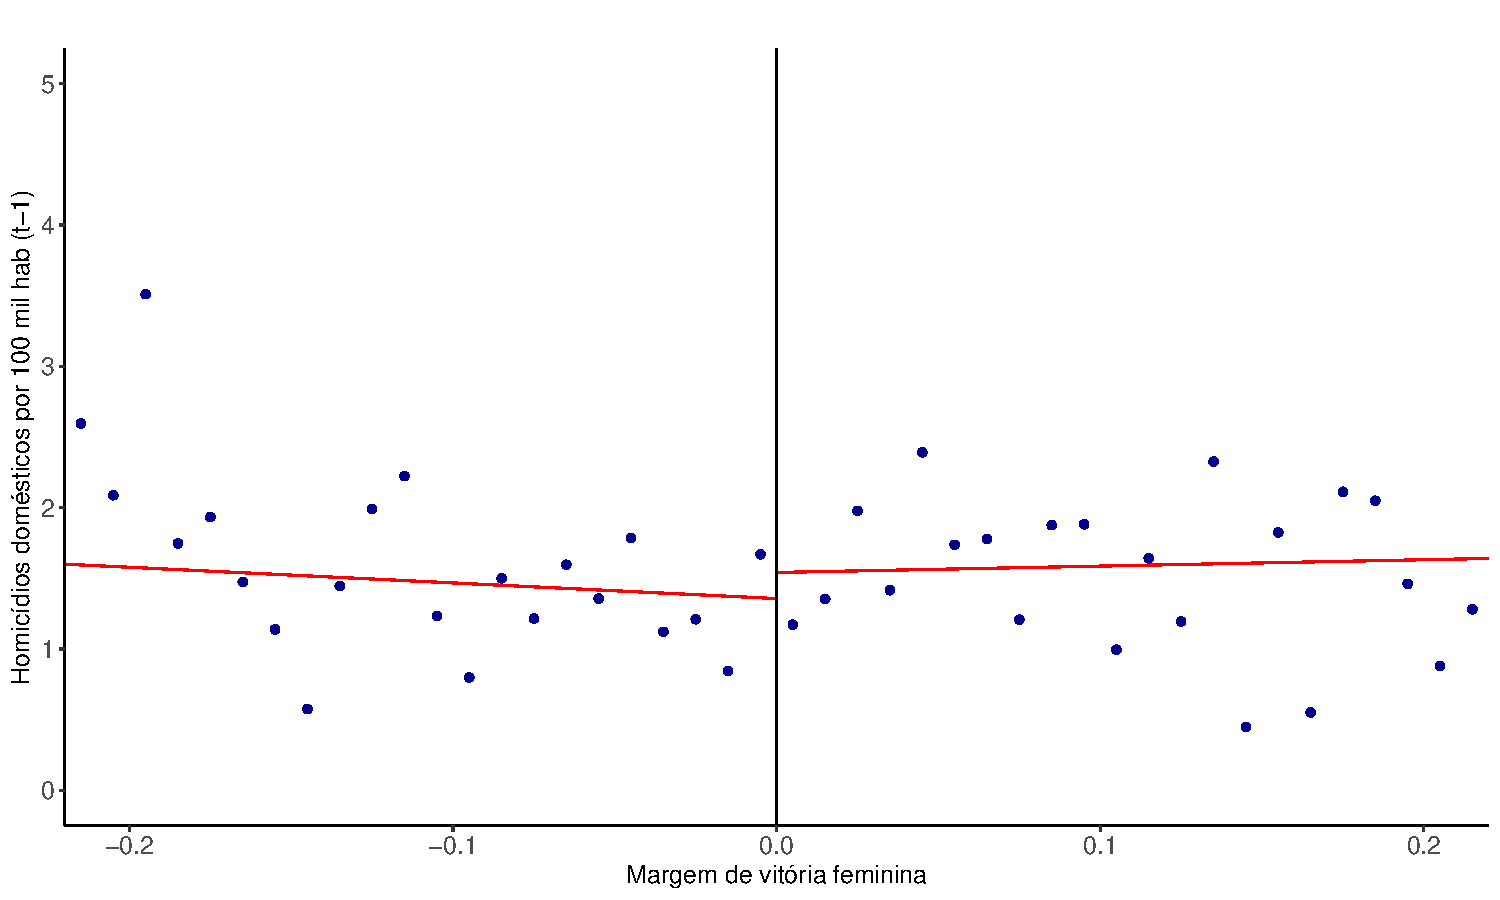
\includegraphics[width=0.8\linewidth]{relatorios/close_elections/graficos/rdd_plot_t_1.pdf}
    \caption{Teste Placebo: Efeito da eleição anterior sobre homicídios domésticos (t-1).}
    \label{fig:rdd_plot_t_1}
\end{figure}

Além disso, a Figura \ref{fig:robustez} apresenta um teste de robustez, demonstrando que o Local Average Treatment Effect (LATE) se dilui a medida que a largura de banda aumenta. O que, novamente, reforça a validade da suposta causalidade encontrada.  


\begin{figure}
    \centering
    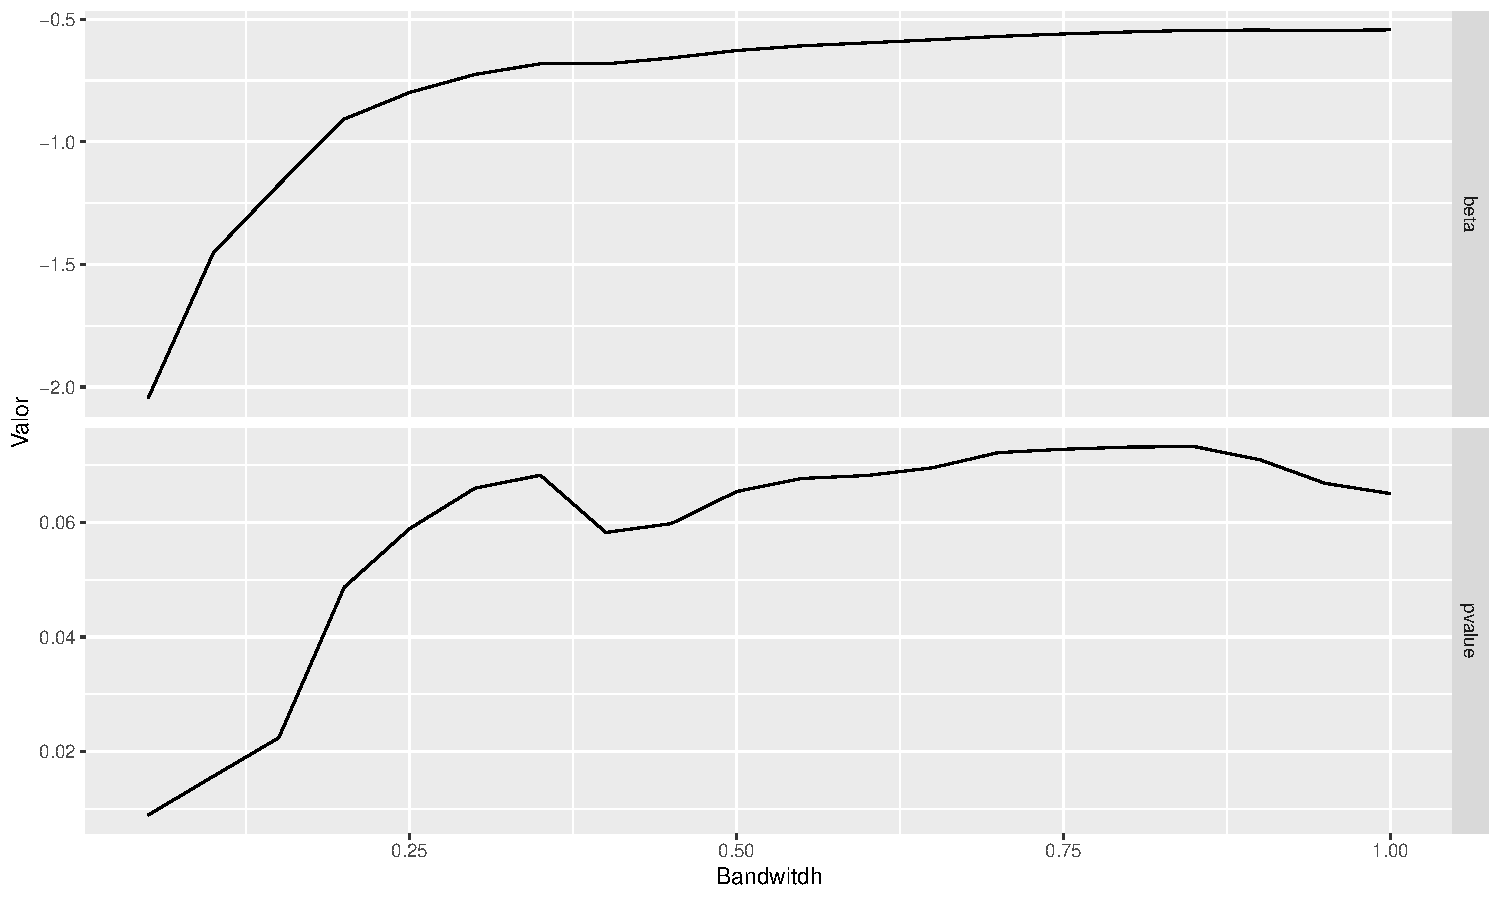
\includegraphics[width=0.8\linewidth]{relatorios/close_elections/graficos/robustez.pdf}
    \caption{Teste de robustez.}
    \label{fig:robustez}
\end{figure}

Em relação às Delegacias Especializadas de Atendimento à Mulher (DEAMs), não foi possível rodar a regressão descontínua para avaliar seu impacto devido ao número reduzido de municípios que implementaram essas delegacias. Como mostrado nas Tabelas \ref{tab:deam_freq} e \ref{tab:distribuicao_genero_ano}, do total de municípios, 577 não possuíam DEAMs em funcionamento durante os três mandatos analisados. Além disso, um número muito pequeno de municípios que apresentaram close elections implementaram as DEAMs durante as eleições de 2004, 2008 e 2012, o que dificultou uma análise estatística robusta. Os detalhes sobre os prefeitos participantes de eleições próximas e que implementaram as DEAMs estão apresentados na Tabela \ref{tab:distribuicao_genero_ano}.

\begin{table}[h]
    \centering
    \begin{tabular}{cc}
        \toprule
        \textbf{Número de DEAMs} & \textbf{Frequência} \\
        \midrule
        0 & 577 \\
        1 & 34 \\
        2 & 4 \\
        \bottomrule
    \end{tabular}
    \caption{Quantidade de DEAMs por município brasileiro}
    \label{tab:deam_freq}
\end{table}


\begin{table}[h]
    \centering
    \begin{tabular}{ccc}
        \toprule
        \textbf{Ano} & \textbf{Mulher eleita} & \textbf{Homem eleito} \\
        \midrule
        2004 & 0 & NA \\
        2008 & 2 & 1 \\
        2012 & 6 & 6 \\
        \bottomrule
    \end{tabular}
    \caption{DEAMs implementadas por prefeitos e prefeitas nos anos analisados}
    \label{tab:distribuicao_genero_ano}
\end{table}


Portanto, a relação entre a presença de DEAMs e a redução dos homicídios domésticos permanece inconclusiva, uma vez que não foi possível estimar esse efeito de maneira estatisticamente válida como planejado no início desta pesquisa.

\section{Conclusão}

A replicação da metodologia utilizada no estudo original confirmou que a eleição de prefeitas leva a uma redução significativa na taxa de homicídios, tanto no âmbito geral quanto no contexto da violência doméstica. Os resultados robustos obtidos pela Regressão Descontínua corroboram a tese de que a representatividade feminina no executivo municipal pode influenciar políticas públicas que reduzem a violência contra as mulheres.

No entanto, a análise das Delegacias Especializadas de Atendimento à Mulher (DEAMs) não permitiu uma conclusão definitiva sobre sua efetividade como canal de combate à violência doméstica. A quantidade insuficiente de municípios com delegacias implementadas impossibilitou a aplicação do método de RDD para estimar o impacto dessas unidades sobre os homicídios. Esse resultado sugere que as DEAMs não são, até o momento, um canal amplamente utilizado para combater a violência doméstica em nível municipal.

Para pesquisas futuras, recomenda-se explorar quais mecanismos específicos são empregados por prefeitas para reduzir a violência de gênero, bem como investigar outras políticas públicas que possam desempenhar esse papel.



\printbibliography[keyword = close-election]
